% !TeX document-id = {f19fb972-db1f-447e-9d78-531139c30778}
% !BIB program = biber
\documentclass{beamer}
%\documentclass[handout]{beamer}

%\usetheme{focus}
%\usepackage[style=authoryear]{biblatex}
%\renewcommand*{\nameyeardelim}{\addcomma\addspace}
\usepackage[T1]{fontenc}
\usetheme[block=fill,subsectionpage=progressbar,sectionpage=none]{metropolis} 
%\usepackage[natbibapa]{apacite}
\usepackage{wasysym}
\usepackage{etoolbox}
\usepackage[utf8]{inputenc}

\usepackage{threeparttable}
\usepackage{subcaption}

\usepackage{tikz-qtree}
\setbeamercovered{still covered={\opaqueness<1->{5}},again covered={\opaqueness<1->{100}}}


\usepackage[american]{babel}
\usepackage{csquotes}
\usepackage[style=apa, backend = biber]{biblatex}
\DeclareLanguageMapping{american}{american-UoN}
\addbibresource{../../bdaca/bdaca.bib}
\graphicspath{{../../bdaca/pictures/}}
\renewcommand*{\bibfont}{\tiny}

\usepackage{tikz}
\usetikzlibrary{shapes,arrows,matrix}
\usepackage{multicol}


\makeatletter
\setbeamertemplate{headline}{%
	\begin{beamercolorbox}[colsep=1.5pt]{upper separation line head}
	\end{beamercolorbox}
	\begin{beamercolorbox}{section in head/foot}
		\vskip2pt\insertnavigation{\paperwidth}\vskip2pt
	\end{beamercolorbox}%
	\begin{beamercolorbox}[colsep=1.5pt]{lower separation line head}
	\end{beamercolorbox}
}
\makeatother



\setbeamercolor{section in head/foot}{fg=normal text.bg, bg=structure.fg}



\newcommand{\question}[1]{
	\begin{frame}[plain]
		\begin{columns}
			\column{.3\textwidth}
			\makebox[\columnwidth]{
				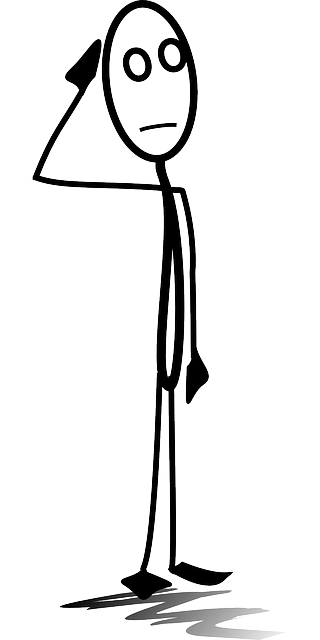
\includegraphics[width=\columnwidth,height=\paperheight,keepaspectratio]{mannetje.png}}
			\column{.7\textwidth}
			\large
			\textcolor{orange}{\textbf{\emph{#1}}}
		\end{columns}
\end{frame}}


\usepackage{listings}

\lstset{
	basicstyle=\scriptsize\ttfamily,
	columns=flexible,
	breaklines=true,
	numbers=left,
	%stepsize=1,
	numberstyle=\tiny,
	backgroundcolor=\color[rgb]{0.85,0.90,1}
}


\title[Big Data and Automated Content Analysis]{\textbf{Teaching the Teacher: Python} \\ Day 1 -- Morning: »Python Basics 1«}
\author[Damian Trilling]{Damian Trilling \\ ~ \\ \footnotesize{d.c.trilling@uva.nl \\@damian0604} \\ \url{www.damiantrilling.net}}
\date{28 June 2021}
\institute[UvA]{Afdeling Communicatiewetenschap \\Universiteit van Amsterdam}

\begin{document}
	
	\begin{frame}{}
		\titlepage
	\end{frame}
	
	\begin{frame}{Today}
		\tableofcontents
	\end{frame}

	
	\section{The toolbox}
	\subsection{The role of software in CSS}
	
	
	
	\begin{frame}{Why program your own tool?}
		\begin{block}{\textcite{Vis2013}}
			``Moreover, the tools we use can limit the range of questions that might be imagined, simply because they do not fit the affordances of the tool. Not many researchers themselves have the ability or access to other researchers who can build the required tools in line with any preferred enquiry. This then introduces serious limitations in terms of the scope of research that can be done.''	
		\end{block}
		
	\end{frame}
	
	
	\begin{frame}{Some considerations regarding the use of software in science}
		Assuming that science should be \emph{transparent} and \emph{reproducible by anyone}\onslide<2->{, we should}
		\begin{block}{use tools that are}<2->
			\begin{itemize}
				\item platform-independent 
				\item free (as in beer and as in speech, gratis and libre)
				\item which implies: open source
			\end{itemize}
		\end{block}
		\onslide<3>{This ensures it can our research (a) can be reproduced by anyone, and that there is (b) no black box that no one can look inside. $\Rightarrow$ ongoing open-science debate! \parencite{VanAtteveldt2019}}
	\end{frame}
	
	\begin{frame}{Why program your own tool?}
		\begin{block}{\textcite{Vis2013}}
			``{[}\ldots{]} these {[}commercial{]} tools are often unsuitable for academic purposes because of their cost, along with the problematic `black box' nature of many of these tools.''
		\end{block}
		
		\begin{block}{\textcite{Mahrt2013}}
			``{[}\ldots{]} we should resist the temptation to let the opportunities and constraints of an application or platform determine the research question {[}\ldots{]}''
		\end{block}
		
	\end{frame}
	
	
	
	
	
	
	\subsection{Python: A language, not a program}
	
	
	\begin{frame}[plain]
		\makebox[\columnwidth]{
			\includegraphics[width=\columnwidth,height=\paperheight,keepaspectratio]{knitting.jpg}}
		\footnotesize{An algorithm in a language that's a bit harder (I think) than Python}
	\end{frame}
	
	
	
	\begin{frame}{Python}
		\begin{block}{What?}<1->
			\begin{itemize}
				\item A language, not a specific program
				\item Huge advantage: flexibility, portability
				\item One of \emph{the} languages for data analysis. \tiny{(The other one is R.)}
				\onslide<2>{ \\\tiny{But Python is more flexible---the original version of Dropbox was written in Python. Some people say: R for numbers, Python for text and messy stuff.}}
			\end{itemize}
		\end{block}
		
		\begin{block}{Which version?}<3->
			We use Python 3. \\ 
			\footnotesize{\url{http://www.google.com} or \url{http://www.stackexchange.com} still may show you some Python2-code, but that can easily be adapted. Most notable difference: In Python 2, you write {\tt print "Hi"}, this has changed to {\tt print ("Hi")}.}\\
		\end{block}
	\end{frame}
	
	\begin{frame}[standout]
		Let's run some Python code together!
	\end{frame}
	
	
	
	
	
	
	\section{Datatypes}
	
	
	\begin{frame}{Python lingo}
		\begin{block}{Basic datatypes (variables)}
			\begin{description}
				\item[{\color{red}int}] \texttt{37}
				\item[{\color{red}float}] \texttt{1.75}
				\item[{\color{red}bool}] \texttt{True}, \texttt{False}
				\item[{\color{red}string}] \texttt{"Alice"}
				\onslide<2->{\scriptsize \item[({\color{red}variable name}] \texttt{firstname})}
			\end{description}
		\end{block}
		\onslide<2->{\textbf{"firstname" and firstname is not the same.\\}}
		\onslide<3->{\textbf{"5" and 5 is not the same.}\\ But you can transform it: {\tt{int("5")}} will return 5.}\\
		\onslide<3->{\textbf{You cannot calculate \texttt{3 * "5"}} {\tiny{(In fact, you can. It's \tt{"555"})}}.\\
			But you can calculate {\tt{3 * int("5")}}}
	\end{frame}
	
	
	
	\begin{frame}{Python lingo}
		\begin{block}{More advanced datatypes}
			\begin{description}
				\item[{\color{red}list}]<2-> \texttt{firstnames = ['Alice','Bob','Cecile'] \\
					lastnames = ['Garcia','Lee','Miller']}
				\item[{\color{red}list}]<3->\texttt{ages = [18,22,45]}
				\item[{\color{red}dict}]<4-> \texttt{agedict = \{'Alice': 18, 'Bob': 22, 'Cecile': 45\} }
			\end{description}
			\onslide<5->{
				Note that the elements of a list, the keys of a dict, and the values of a dict can have any* datatype! (You can even mix them, but it's better to be consistent!)
				
				\tiny{*Well, keys cannot be mutable $\rightarrow$ see book}}
		\end{block}
	\end{frame}
	
	
	\begin{frame}{Python lingo}
		\begin{block}{Retrieving specific items}
			\begin{description}
				\item[{\color{red}list}]<1-> \texttt{firstnames[0]} gives you the first entry\\ 
				\texttt{firstnames[-2]} gives you the one-but-last entry\\
				\texttt{firstnames[:2]} gives you entries 0 and 1\\
				\texttt{firstnames[1:3]} gives you entries 1 and 2\\
				\texttt{firstnames[1:]} gives you entries 1 until the end\\
				\item[{\color{red}dict}]<2-> \texttt{agedict["Alice"]} gives you 18 
			\end{description}
			
		\end{block}
	\end{frame}
	
	
	\question{Think of at least two different ways of storing data about some fictious persons (first name, last name, age, phone number, \ldots) using lists and/or dictionaries. What are the pros and cons?}
	
	
	\begin{frame}{Python lingo}
		\begin{block}{Less frequent, but still useful datatypes}
			\begin{description}
				\item[{\color{red}set}]A collection in which each item is unique: \texttt{\{1,2,3\}}
				\item[{\color{red}tuple}]Like a list, but \emph{immutable}: \texttt{(1,2,2,2,3)}
				\item[{\color{red}defaultdict}]A dict that does not raise an error but returns the ``empty'' value of its datatype (0 for int, "" for str) if you try access a non-existing key (great for storing results and counting things!)
				\item[{\color{red}np.array}]A list-like datatype provided by the \texttt{numpy} package optimized for efficient mathematical operations.
				\item[$\ldots$]\ldots
			\end{description}
		\end{block}
		\small{You will come across more later}
	\end{frame}
	
	
	
	\section{Functions and methods}
	\begin{frame}{Python lingo}
		\begin{block}{Functions}
			\begin{description}
				\item[{\color{red}functions}]<2-> Take an input and return something else \\ {\tt{int(32.43})} returns the integer 32. \texttt{len("Hello")} returns the integer 5.\\ 
				\item[{\color{red}methods}]<3-> are similar to functions, but directly associated with an object. {\tt{"SCREAM".lower()}} returns the string "scream"
			\end{description}
		\end{block}
		\onslide<4->{Both functions and methods end with \texttt{()}. Between the \texttt{()}, \emph{arguments} can (sometimes have to) be supplied.}
	\end{frame}
	
	
	
	\begin{frame}[fragile]{Some functions}
\begin{lstlisting}
len(x)        # returns the length of x
y = len(x)    # assign the value returned by len(x) to y
print(len(x)) # print the value returned by len(x)
print(y)      # print y
int(x)        # convert x to an integer
str(x)        # convert x to a string
sum(x)        # get the sum of x
\end{lstlisting}
	\end{frame}
	
	\question{How could you print the mean (average) of a list of integers using the functions on the previous slide?}
	


\begin{frame}[fragile]{Some methods}
Some string methods
\begin{lstlisting}
mystring = "Hi! How are you?"
mystring.lower()   # return lowercased string (doesn't change original!)
mylowercasedstring =  mystring.lower()  # save to a new variable
mystring =  mystring.lower()  # or override the old one
mystring.upper()   # uppercase
mystring.split()   # Splits on spaces and returns a list ['Hi!', 'How', 'are', 'you?']
\end{lstlisting}

	We'll look into some list methods later.
	
	\textbf{$\Rightarrow$ You can use TAB-completion in Jupyter to see all methods (and properties) of an object!}
\end{frame}


\begin{frame}[fragile]{Writing own functions}
You can write an own function:
\begin{lstlisting}
def addone(x):
    y = x + 1
    return y
\end{lstlisting}

Functions take some input (``argument'') (in this example, we called it \texttt{x}) and \emph{return} some result.

Thus, running
\begin{lstlisting}	
addone(5)
\end{lstlisting}
returns \tt{6}.
\end{frame}

\begin{frame}[fragile]{Writing own functions}

\begin{alertblock}{Attention, R users! (maybe obvious for others?)}
	You \emph{cannot}* apply the function that we just created on a whole list -- after all, it takes an int, not a list as input.
\end{alertblock}

(wait a sec foruntil we cover for loops later today, but this is how you'd do it (by calling the function for each element in the list separately):):

\begin{lstlisting}
mynumbers = [5, 3, 2, 4]
results = [addone(e) for e in mynumbers]
\end{lstlisting}

\vspace{1cm}
\tiny{* Technically speaking, you could do this by wrapping the \texttt{map} function around your own function, but that's not considered ``pythonic''. Don't do it ;-) \\}
\end{frame}


	

\section[Modifying lists \& dicts]{Modifying lists and dictionaries}
\begin{frame}[fragile]{Modifying lists}
Let's use one of our first \textcolor{red}{method}s! Each \emph{list} has a method \texttt{.append()}:
\begin{block}{Appending to a list}
\begin{lstlisting}
mijnlijst = ["element 1", "element 2"]
anotherone = "element 3"   # note that this is a string, not a list!
mijnlijst.append(anotherone)
print(mijnlijst)
\end{lstlisting}
gives you:
\begin{lstlisting}
["element 1", "element 2", "element 3"]
\end{lstlisting}
\end{block}
\end{frame}



\begin{frame}[fragile]{Modifying lists}
\begin{block}{Merging two lists (= extending)}
\begin{lstlisting}
mijnlijst = ["element 1", "element 2"]
anotherone = ["element 3", "element 4"]
mijnlist.extend(anotherone)
print(mijnlijst)
\end{lstlisting}
gives you:
\begin{lstlisting}
["element 1", "element 2", "element 3", "element 4]
\end{lstlisting}
\end{block}
\end{frame}

\question{What would have happened if we had used \texttt{.append()} instead of \texttt{.extend()}?}

\question{Why do you think that the Python developers implemented \texttt{.append()} and \texttt{.extend()} as methods of a list and not as functions?}


\begin{frame}[fragile]{Modifying dicts}
\begin{block}{Adding a key to a dict (or changing the value of an existing key)}
\begin{lstlisting}
mydict = {"whatever": 42, "something": 11}
mydict["somethingelse"] = 76
print(mydict)
\end{lstlisting}
gives you:
\begin{lstlisting}
{'whatever': 42, 'somethingelse': 76, 'something': 11}
\end{lstlisting}
If a key already exists, its value is simply replaced.
\end{block}
\end{frame}




\section{for, if/elif/else, try/except}

\begin{frame}[fragile]{How can we structure our program?}
If we want to \emph{repeat} a block of code, exectute a block of code only \emph{under specific conditions}, or more generally want to structure our code, we use \emph{indention}.

\begin{block}{Indention: The Python way of structuring your program}
	\begin{itemize}
		\item Your program is structured by TABs or SPACEs.
		\item Jupyter (or your IDE) handles (guesses) this for you, but make sure to not interfere and not to mix TABs or SPACEs!
		\item Default: four spaces per level of indention.
	\end{itemize}
\end{block}
\end{frame}



\begin{frame}[fragile]{Indention}
\begin{block}{Structure}
	A first example of an indented block -- in this case, we want to \emph{repeat} this block:
\end{block}
\begin{lstlisting}
agedict = {'Zeus': None, 'Denis': 96, 'Alice': 18, 'Rebecca': 20 , 'Bob': 22, 'Cecile': 45}

myfriends = ['Alice','Bob','Cecile']

print ("The names and ages of my friends:")
for buddy in myfriends:
  print (f"My friend {buddy} is {agedict[buddy]} years old")
\end{lstlisting}

Output:
\begin{lstlisting}
My friend Alice is 18 years old
My friend Bob is 22 years old
My friend Cecile is 45 years old
\end{lstlisting}
\end{frame}

\begin{frame}[fragile]{What happened here?}

\begin{lstlisting}
for buddy in myfriends:
    print (f"My friend {buddy} is {agedict[buddy]} years old")
\end{lstlisting}

\small
\begin{block}{The for loop}
	\begin{enumerate}
		\item Take the first element from \texttt{myfriends} and call it \texttt{buddy} (like \texttt{buddy = myfriends[0]}) (line 1)
		\item Execute the indented block (line 2, but could be more lines)
		\item Go back to line 1, take next element  (like \texttt{buddy = myfriends[1]}) 
		\item Execture the indented block \ldots
		\item \ldots repeat until no elements are left \ldots
	\end{enumerate}
\end{block}

\begin{block}{The f-string (\emph{formatted} string)}
	If you prepend a string with an \texttt{f}, you can use curly brackets \texttt{\{\}} to insert the value of a variable
\end{block}

\end{frame}




\begin{frame}[fragile]{What happened here?}
\begin{lstlisting}
for buddy in myfriends:
    print (f"My friend {buddy} is {agedict[buddy]} years old")
\end{lstlisting}
\small
The line \emph{before} an indented block starts with a \emph{statement} indicating what should be done with the block and ends with a \texttt{:}

\footnotesize
\begin{block}{More in general, the \texttt{:} + indention indicates that}<2->
	\begin{itemize}
		\item<3-> the block is to be executed repeatedly (\texttt{for} statement) – e.g., for each element from a list, or until a condition is reached (\texttt{while} statement)
		\item<4-> the block is only to be executed under specific conditions (\texttt{if}, \texttt{elif}, and \texttt{else} statements)
		\item<5-> an alternative block should be executed if an error occurs in the block (\texttt{try} and \texttt{except} statements)
		\item<6-> a file is opened, but should be closed again after the block has been executed (\texttt{with} statement)
	\end{itemize}
\end{block}
\end{frame}



\begin{frame}[fragile]{Can we also loop over dicts?}
Sure! But we need to indicate how exactly:

\begin{lstlisting}
mydict = {"A":100, "B": 60, "C": 30}

for k in mydict:   # or mydict.keys()
  print(k)

for v in mydict.values():
  print(v)

for k,v in mydict.items():
  print(f"{k} has the value {v}")
\end{lstlisting}

\end{frame}




\begin{frame}[fragile]{Can we also loop over dicts?}
The result:

\begin{lstlisting}
A
B
C

100
60
30

A has the value 100
B has the value 60
C has the value 30
\end{lstlisting}

\end{frame}



\begin{frame}[fragile]{if statements}
\begin{block}{Structure}
	Only execute block if condition is met
\end{block}
\begin{lstlisting}
x = 5
if x <10:
  print(f"{x} is smaller than 10")
elif x > 20:
  print(f"{x} is greater than 20")
else:
  print("No previous condition is met, therefore 10<={x}<=20")
\end{lstlisting}

\end{frame}


\question{Can you see how such an if statement could be particularly useful when nested in a for loop?}



\begin{frame}[fragile]{try/except}
\begin{block}{Structure}
	If executed block fails, run another block instead
\end{block}
\begin{lstlisting}
x = "5"
try: 
  myint = int(x)
except:
  myint = 0
\end{lstlisting}

\pause 
\small{Again, more useful when executed repeatedly (in a loop or function):}
\begin{lstlisting}
mylist = ["5", 3, "whatever", 2.2]
myresults = []
for x in mylist:
  try: 
    myresults.append(int(x))
  except:
    myresults.append(None)
print(myresults)
\end{lstlisting}
\end{frame}





\section{Bonus: Python goodies}

\begin{frame}[fragile]{List comprehensions}
\begin{block}{Structure}
A for loop that \texttt{.append()}s to an empty list can be replaced by a one-liner:
\end{block}
\begin{lstlisting}
mynumbers = [2,1,6,5]
mysquarednumbers = []
for x in mynumbers:
    mysquarednumbers.append(x**2))
\end{lstlisting}
is equivalent to:
\begin{lstlisting}
mynumbers = [2,1,6,5]
mysquarednumbers = [x**2 for x in mynumbers]
\end{lstlisting}

\pause 
Optionally, we can have a condition:
\begin{lstlisting}
mynumbers = [2,1,6,5]
mysquarednumbers = [x**2 for x in mynumbers if x>3]
\end{lstlisting}

\end{frame}




\begin{frame}[fragile]{List comprehensions}
\begin{alertblock}{A very pythonic construct}
\begin{itemize}
\item Every for loop can also be written as a for loop that appends to a new list to collect the results. 
\item For very complex operations (e.g., nested for loops), it can be easier to write out the full loops. 
\item But mostly, list comprehensions are really great! (and much more concise!)
\end{itemize}
\end{alertblock}
\textbf{$\Rightarrow$ You really should learn this!}
\end{frame}




\begin{frame}[plain]
\printbibliography
\end{frame}

\end{document}
